% Szglab4
% ===========================================================================
%
\chapter{Szkeleton tervezése}

\thispagestyle{fancy}

\section{A szkeleton modell valóságos use-case-ei}
\comment{A szkeletonnak, mint önálló programnak a működésével kapcsolatos use-case-ek.}

\subsection{Use-case diagram}

\begin{figure}[h]
\begin{center}
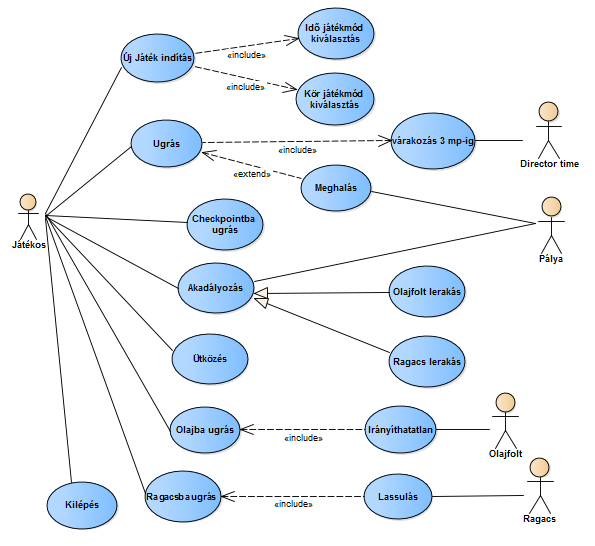
\includegraphics[width=17cm]{skeleteon_use_case2.PNG}
\caption{x}
\label{fig:SzkeletonUseCase}
\end{center}
\end{figure}
\newpage

\subsection{Use-case leírások}
\comment{Szerintem bele lehetne venni a use-case-ekbe még a "robottal való ütközés"-t és a "checkpoint-ba ugrás"-t is. //Winnie}
\comment{Egyetértek, javítva, megoldva! ;) //Attó}

\usecase{Új játék indítása}{A játékos elindítja a játékot.}{Játékos}{A grafikus felületen (menüben) a felhasználó rákattinthat az „Új Játék indítása” menüpontra.}
\usecase{Idő játékmód kiválasztása}{A játékos kiválasztja az idő játékmódot.}{Játékos}{A grafikus felületen (menüben) a felhasználó olyan játékmódban indítja el a játékot amiben egy számláló fut visszafelé, és ha lejár, vége a játéknak.}
\usecase{Kör játékmód kiválasztása}{A játékos kiválasztja a kör játékmódot.}{Játékos}{A grafikus felületen (menüben) a felhasználó olyan játékmódban indítja el a játékot, melyben el kell érni egy megadott körszámot, és ezután ér véget a játék.}
\usecase{Ugrás}{A robot ugrik a megadott irányba.}{Játékos}{A játékos a megadott billentyűkkel beállítja az ugrás irányát, majd a robot ugrik.}
\usecase{Várakozás 3mp-ig}{Egy számláló 3 másodpercig visszaszámol.}{Director time}{A körökre osztás miatt a robot csak három másodpercenként ugrik.}
\usecase{Meghalás}{A robot meghal.}{Pálya}{Az ugrás után, ha a robot nem tartózkodik a pályán, akkor meghal.}
\newpage
\usecase{Akadályozás}{A pályára akadályok kerülnek.}{Játékos, Pálya}{A játékos utasíthatja a robotot, hogy rakjon le akadályt a pályára, illetve a pályára is kerülnek akadályok a játék elején.}
\usecase{Ragacs lerakás}{A pályára ragacs kerül.}{Játékos}{A robot ragacsot rak le a pályára a játékos utasítására.}
\usecase{Olajfolt lerakás}{A pályára olajfolt kerül.}{Játékos}{A robot olajfoltot rak le a pályára a játékos utasítására.}
\usecase{Olajba ugrás}{A játékos olajfoltba ugrik.}{Játékos}{A robot az ugrás után egy olajfoltra érkezik a pályán.}
\usecase{Irányíthatatlan}{A robot irányíthatatlan lesz.}{Olajfolt}{A játékos nem fogja tudni megváltoztatni a következő körben a robot ugrásának irányát, az „csúszni” fog tovább.}
\usecase{Ragacsba ugrás}{A játékos ragacsba ugrik.}{Játékos}{A robot az ugrás után egy ragacsba érkezik a pályán.}
\usecase{Lassulás}{A robot sebessége a felére csökken.}{Ragacs}{Ha a robot ragacsba ugrik a pályán, akkor sebessége a felére csökken, a következő körben nem tud akkorát ugrani.}
\newpage
\usecase{Kilépés}{A játékos kilép a játékból.}{Játékos}{A felhasználó visszalép a menübe, vagy teljesen leállítja a játék működését.}


\section{A szkeleton kezelői felületének terve, dialógusok}
\comment{A szkeleton által elfogadott bemenetek , valamint a szöveges konzolon megjelenő kimenetek. A kiemenet formátuma olyan kell legyen, ami alapján a működés összevethető a korábbi szekvencia-diagramokkal.}

\section{Szekvencia diagramok a belső működésre}
\comment{A szkeletonban implementált szekvenciadiagramok. Tipikusan egy use-case egy diagram. Ezek megegyezhetnek a korábban specifikált diagramokkal, de az egyes életvonalakat (lifeline) egyértelműen a szkeletonban példányosított objektumokhoz kell tudni kötni. Azt kell megjeleníteni, hogy a szkeletonban létrehozott objektumok egymással hogyan fognak kommunikálni.}

\section{Kommunikációs diagramok}
\comment{A szkeletonban, az egyes szkeleton-use-case-ek futása során létrehozott objektumok és kapcsolataik bemutatására szolgáló diagramok. Ezek alapján valósítják meg a szkeleton fejlesztői az inicializáló kódrészleteket.}
